Una idea muy trivial para solucionar el problema pudiera ser para cada nodo del árbol buscar buscar su nodo mas alejado y la solución sería aquel par de nodos cuya distancia entre ellos fuera mayor. Esto lo pudieramos realizar aplicando un dfs por cada nodo lo cual podría tener una complejidad de O($VE$) siendo $V$ la cantidad de nodos y $E$ la cantidad de aristas del árbol, pero como la cantidad de aristas de un árbol es igual a $V-1$ la complejidad de esta solución quedaría O($V^2-V$). Pero esta idea tan trivial es la que da inicio a la primera variante de solución.

\subsection{Recorrido en Profundidad (\emph{DFS})}

El algoritmo en sí mismo es bastante simple. Se toma un nodo $a$ de forma aleatoria y se explora el resto del árbol usando un dfs y calculando para cada nodo del árbol su distancia con respecto al nodo $a$ . Una vez terminado este primer dfs buscamos que nodo esta más alejado con respecto al nodo $a$  que tomamos de forma aleatoria la primera vez. Al nodo mas alejado del nodo $a$  lo nombraremos nodo $b$ . Ahora a partir del nodo $b$  realizaremos un dfs para buscar el nodo $c$  que va ser el nodo más alejado del nodo $b$ . Una vez hallado el nodo $c$ , podemos decir con seguridad que el par de nodos $b,c$  son los nodos más alejados en el árbol por tanto su distancia entre ellos va a definir el díametro del árbol.

En el siguiente árbol, $a$, $b$ y $c$ podrían ser:

\begin{figure}[h!]
	\centering
	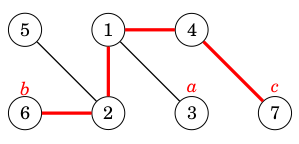
\includegraphics[width=0.5\linewidth]{img/diameter_tree_3}
	\label{fig:diametertree3}
\end{figure}

Este es un método elegante, pero ¿por qué funciona?

Ayuda dibujar el árbol de manera diferente para que el camino que corresponde al diámetro sea horizontal y todos los demás nodos cuelguen de él:

\begin{figure}[h!]
	\centering
	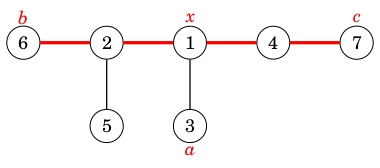
\includegraphics[width=0.5\linewidth]{img/diameter_tree_4}
	\label{fig:diametertree4}
\end{figure}

El nodo $x$ indica el lugar donde el camino del nodo $a$ se une al camino que corresponde al diámetro. El nodo más alejado de $a$ es el nodo $b$, el nodo $c$ o algún otro nodo que esté al menos tan lejos del nodo $x$. Por lo tanto, este nodo es siempre una opción válida para un punto final de una trayectoria que corresponde al diámetro.

\subsection{Programación Dinámica}

Una forma general de abordar muchos problemas de árboles es enraizar primero el árbol de forma arbitraria. Después de esto, podemos intentar resolver el problema por separado para cada subárbol. El siguiente algoritmo para calcular el diámetro se basa en esta idea.

Una observación importante es que cada camino en un árbol enraizado tiene un punto más alto: el nodo más alto que pertenece al camino. Así, podemos calcular para cada nodo la longitud del camino más largo cuyo punto más alto es el nodo. Uno de esos caminos corresponde al diámetro del árbol.

Por ejemplo, en el siguiente árbol, el nodo 1 es el punto más alto del camino que corresponde al diámetro:

\begin{figure}[h!]
	\centering
	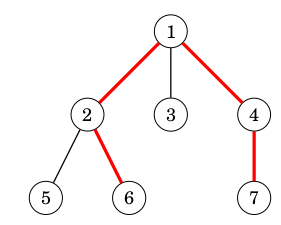
\includegraphics[width=0.5\linewidth]{img/diameter_tree_5}
	\label{fig:diametertree5}
\end{figure}

Calculamos para cada nodo $x$ dos valores:

\begin{itemize}
	\item \textbf{toLeaf(x):} La longitud máxima de una ruta desde $x$ a cualquier hoja
	\item \textbf{maxLength(x):} La longitud máxima de un camino cuyo punto más alto es $x$.
\end{itemize}

Por ejemplo, en el árbol anterior, $toLeaf(1) = 2$, porque hay una ruta $1 \rightarrow 2 \rightarrow 6$, y $maxLength(1) = 4$, porque hay una ruta $6 \rightarrow 2 \rightarrow 1 \rightarrow 4 \rightarrow 7$. En En este caso, $maxLength(1)$ es igual al diámetro.

La programación dinámica se puede utilizar para calcular los valores anteriores para todos los nodos en tiempo O($n$). Primero, para calcular $toLeaf(x)$, revisamos los hijos de $x$, elegimos un hijo $c$ con $toLeaf(c)$ máximo y sumamos uno a este valor. Luego, para calcular $maxLength(x)$, elegimos dos hijos distintos $a$ y $b$ tales que la suma $toLeaf(a) + toLeaf(b)$ sea máxima y sumamos dos a esta suma
